In this chapter there will be described expected behavior of product and its resulting requirements. 
First there will be introduced simple life cycle of the product.
Although project title was accepted as a domain and not a final product, following requirements could be applied also on project that is not scaled down.

\section{Description}
To clarify and properly explain life cycle of one run of server side application, its usage and possible requirements, structure of UML's activity diagram was adopted. 
Therefore we show in figure \ref{img:activity_diagram} interaction between manager and one client user.
Notice that there are some actions of both Manager and client user which do require direct manipulation with mobile phone or other actors such as "Notice users to raise their mobiles", "Raise mobile", "Put down mobile" and more.

\begin{figure}[h!]
    
    \begin{center}
    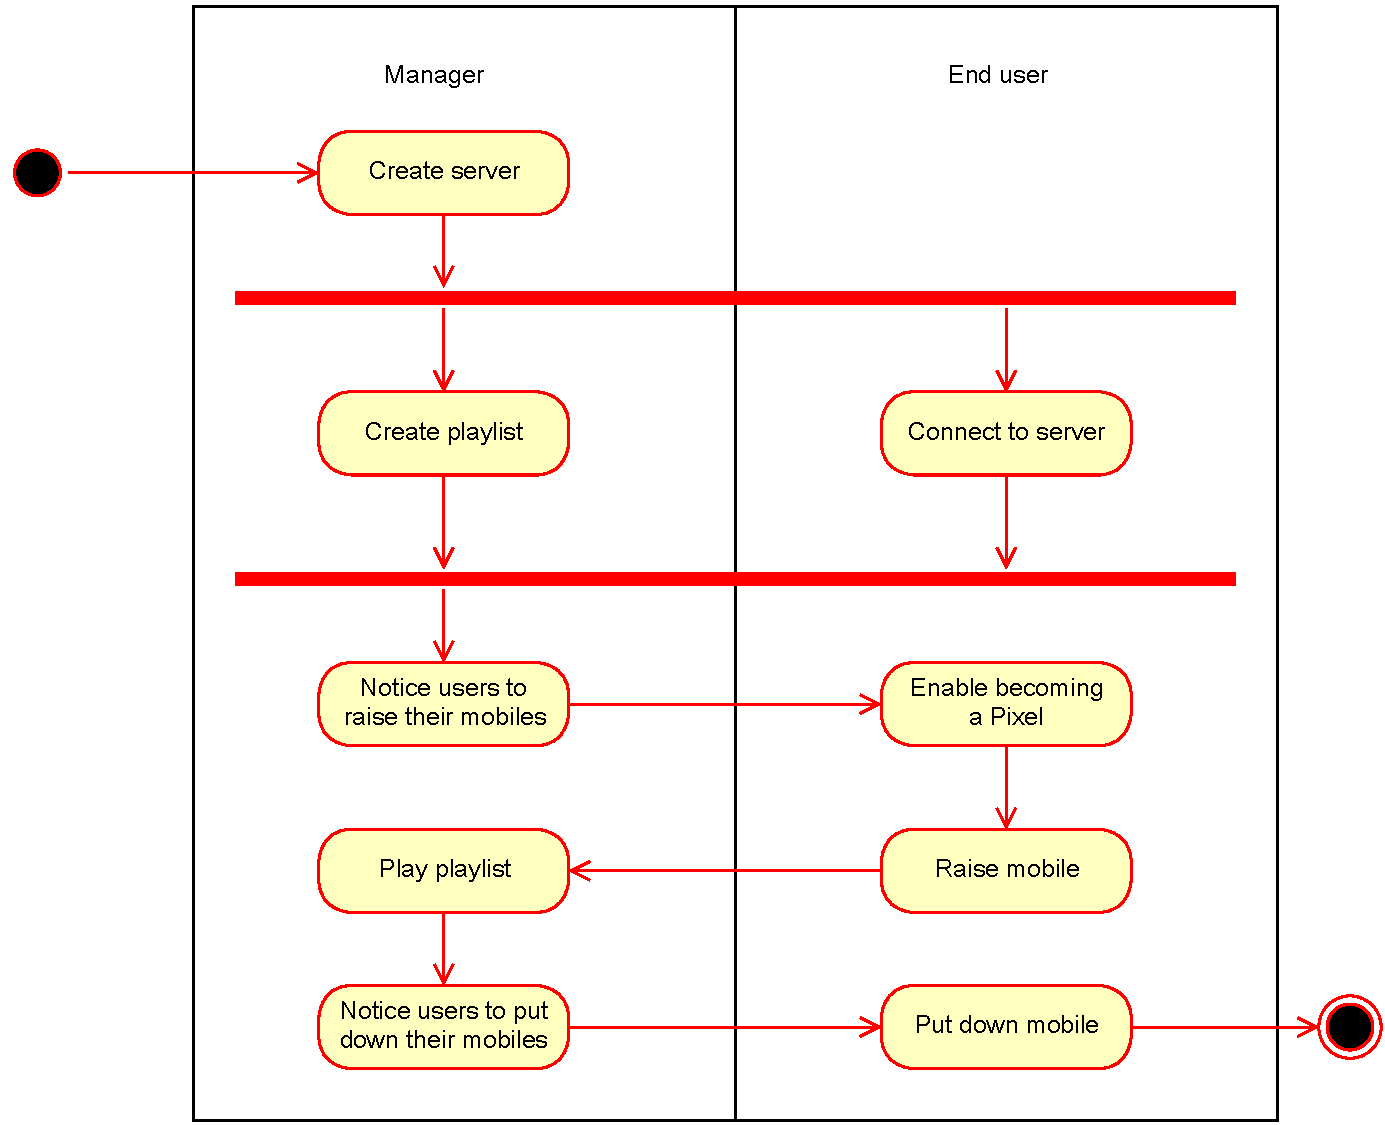
\includegraphics[scale=0.4]{images/activity_diagram.pdf}
    \label{img:activity_diagram}
    \caption{Activity diagram depicting basic scenario of using product with all actors.}
    \end{center}
\end{figure}


\section{Use case diagram}
As we have defined terminology in section \ref{sec:terminology} we will use actor's names according to that terminology.
In the figure bellow is shown use case diagram \ref{img:usecase} of the whole system.

\begin{figure}[h!]
    \begin{center}
    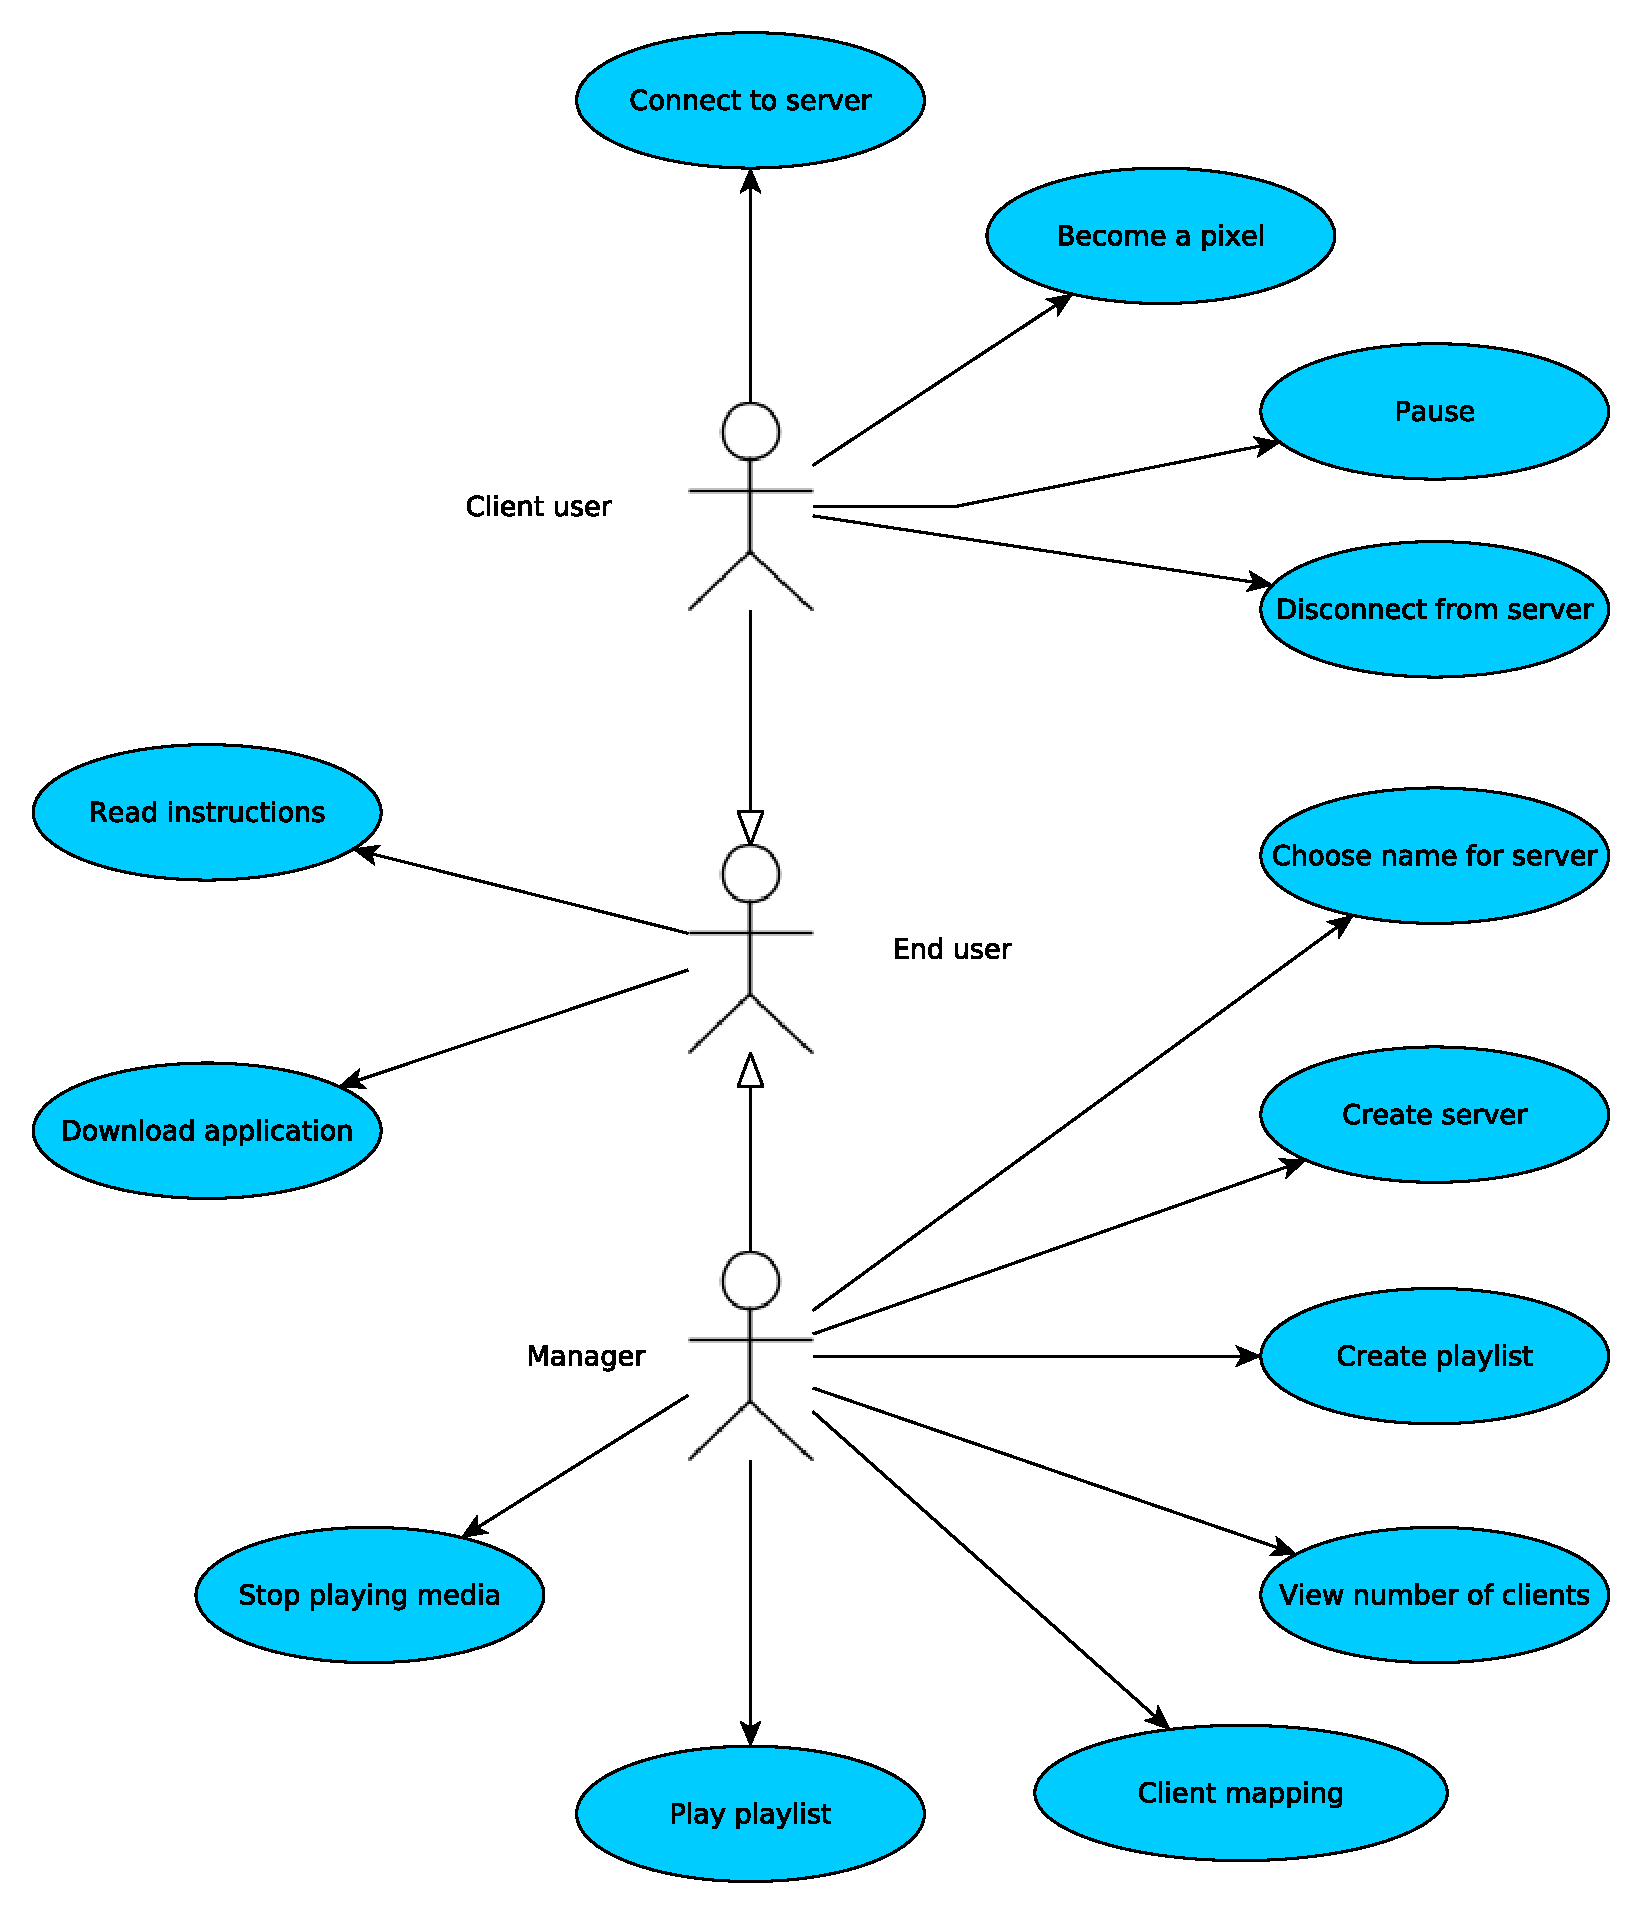
\includegraphics[scale=0.4]{images/usecase.pdf}
    \caption{Use case diagram depicting all actors.}
    \label{img:usecase}
    \end{center}
\end{figure}

\section{Requirements}
Requirements can be divided into two categories - functional and non-functional. 
Functional ones describe what should product do, its specific behavior or function.
On the other hand non-functional requirements cover what product is.


\subsection{Functional}
According to use case diagram \ref{img:usecase}, functional requirements were created.
You can see list of those requirements from end user's point of view below.

\begin{enumerate}
	\item[\textbf{E1}] \label{req_E1}
		I as a end user want to be able to read instructions.
	\item[\textbf{E2}] \label{req_E2}
		I as a end user want to be able to download relevant application from mobile application store.
\end{enumerate}

You can see list of functional requirements from client user's point of view below.
\begin{enumerate}
	\item[\textbf{C1}] \label{req_C1}
		I as a client user I want to easily choose to which server/concert stage I would like to connect.
	\item[\textbf{C2}] \label{req_C2}
		I as a client user I want to connect to chosen server.
	\item[\textbf{C3}] \label{req_C3}
		I as a client user I want to become a \emph{Pixel}.
	\item[\textbf{C4}] \label{req_C4}
		I as a client user I want to be able to pause being a Pixel.
	\item[\textbf{C5}] \label{req_C5}
		I as a client user I want to be able to disconnect from server/stage.
\end{enumerate}


You can see list of functional requirements from manager's point of view below.
\begin{enumerate}
	\item[\textbf{M1}] \label{req_M1}
		I as a manager I want to be able to choose name for my server/stage.
	\item[\textbf{M2}] \label{req_M2}
		I as a manager I want to be able to create a server.
	\item[\textbf{M3}] \label{req_M3}
		I as a manager I want to be able view attendance.
	\item[\textbf{M4}] \label{req_M4}
		I as a manager I want to be able to start mobile phone localization.
	\item[\textbf{M5}] \label{req_M5}
		I as a manager I want to be able to choose playlist to be played.
	\item[\textbf{M6}] \label{req_M6}
		I as a manager I want to be able to start playing given media.
	\item[\textbf{M7}] \label{req_M7}
		I as a manager I want to be able to start pause playing the media.
	\item[\textbf{M8}] \label{req_M8}
		I as a manager I want to be able to start pause stop the media.
\end{enumerate}

\subsubsection{Detailed use cases}
In this section there will be described some use cases in detail.
\begin{table*}[!h]
	\def\arraystretch{1.25}
	\caption{Use case detail: Create playlist}
	\label{tab:usecase1}
	
	\begin{tabular}{p{\textwidth}}
		\toprule
		\textbf{Use case detail: Create playlist} \\
		\midrule
		Actors: Manager \\
		Conditions:
		\begin{enumerate}
			\item Manager had created server.
		\end{enumerate}
		Events flow:
		\begin{enumerate}
			\item Use case starts when manager choose option "Create playlist".
			\item Application will display list of possible media (videos, images) that can be played.
			\item Manager can preview specific media (view on his own screen).
			\item Manager chooses media to be played, order of choosing will be order of playing.
			\item Manager confirms the playlist.
			\item Use case ends.
		\end{enumerate}
		Alternative flow:
		\begin{enumerate}
			\item Manager can quit the screen and return to main menu anytime.
		\end{enumerate}
%		\\ 
		\vspace{0.6em}
		\hrule
%		\\[0.1pt]
%		\bottomrule[1mm]
	\end{tabular}
\end{table*}

\subsection{Non-functional}
You can see non-functional requirements listed below.

\begin{enumerate}
\item[\textbf{N1}] \label{req_N1} Product must work as a server and client architecture.
\item[\textbf{N2}] \label{req_N2} Client side application must work on at least one mobile platform.
\item[\textbf{N3}] \label{req_N3} Application must be deployed to relevant mobile application store.
\item[\textbf{N4}] \label{req_N4} The product must be scalable - it must work with different count of mobile phones.
\item[\textbf{N5}] \label{req_N5} The product must be prepared for future using outside of rock concert domain.
\item[\textbf{N6}] \label{req_N6} Final product must be finished until 21st of November 2013 and presented to the committee and the customer.
\end{enumerate}

\subsubsection{Quality attributes}

\paragraph{Accessibility}
Accessibility is the degree to which a the product is available to as many people as possible. 
Accessibility can be viewed as the "ability to access" and benefit from the product. 
To achieve this we plan to release the product on the Android appstore, and we are also using Testflight to make the applications as accessible as we can.

\paragraph{Availability}

Availability is the ability to be available for use, especially if faults occur. Faults must be recognized or avoided and so the system must react in a particular way. What happens depends on what we want. Ignore. Continue as before. Recovery is the combination of retry and maintain. Prevent is clear. To achieve this requirement must be aware of the faults that may occur and generate response.

\paragraph{Interoperability}
Interoperability refers to the ability of the product to usefully exchange information. The client-server architecture must have the intention of exchanging information. 

WRITE MORE

\paragraph{Maintainability}
Maintainability is the ease with which a product can be maintained. This means the product needs to isolate defects or their cause, prevent unexpected breakdowns, correct defects and repair or replace faulty components. If one component need to be replaced, then the system should do this without having to replace still-working parts. The product also needs make future maintenance easy.

\paragraph{Modifiability}

Modifiability is all about handling changes, and this is including the extent to which this modification affects other functions. 
We must be prepared for changes, and we can do this  by increase cohesion, and reduce coupling in our product. 
If we make the modules smaller, we will reduce the risk if we have to make a change. 
We can also make sure that we are restricting the dependencies. 
Increasing the cohesion, or interdependency within modules, can affect build time, load time, initialization time or run time.

\paragraph{Performance}
Performance is about managing system resources in the face of particular types of demands to achieve acceptable timing behavior. 
Performance can be measured in terms of throughput and latency. 
Performance can be improved by reducing demand, or by managing resources more appropriately. 
Reducing demands will have the side effect of reducing fidelity, or refuse service to some requests. 
Managing the resources more fitting can be done through scheduling, relication, or simply increase the resources available.

WRITE MORE HERE WEHN WE KNOW MORE!!

\paragraph{Scalability}
 Scalability describes the capability to cope and perform under an increased or expanding workload. A system that scales well will be able to maintain, or even increase its level of performance, or efficiency when tested by larger operational demands.
 If our server works properly with ten clients, but with a thousand clients it might fail to meet response time requirements.
 In our case the average response time probably scales linearly with the number of clients.
 WRITE MORE HERE WEHN WE KNOW MORE!!

\paragraph{Testability}

To ensure that the product testd has payoffs in terms of the cost of testing and reliability of the system. The test harness is software system that isolates testing resources to test cases and test infrastructure so we can easily re-apply tests. Another thing is the creation of test cases prior to the development of a component as developers know which test component must pass. Checking observing system state is a large class of testability tactics. Making it possible to do fault injection, to record system state that the partition key, to isloere from the environment. Complex systems are difficult to test because they have large state space in which contexts where computation takes place, and because the greater the number of number of interconnections among elements of the system. Consistently, the system simply is another tactic that supports testabilitet.

\paragraph{Usability}
Usability is the ease of use and learnability of the product.
Usability includes methods of measuring usability, such as analysis of needs or the study of the principles behind an object's perceived efficiency or elegance. We want our product to be easy to use, understandable, and easy to learn.  

\section{Summary}
In this chapter was explained how the application's basic life-cycle looks like and there was introduced Use case diagram \ref{img:usecase}.
According to Use case diagram \ref{img:usecase} there were created \emph{Epics} which serve as a requirements. 
After that non-functional requirements were introduced.
In following chapters each user story which is connected to relevant requirement will be referenced with requirement's identification.

As you could see, client user's interaction with both applications is rather simple (and as our customer suggested the user interface is not core of the work) the main attention will be focused on image processing, network programming and mapping devices into screen.

\begin{figure}[!ht]
    \begin{center}
    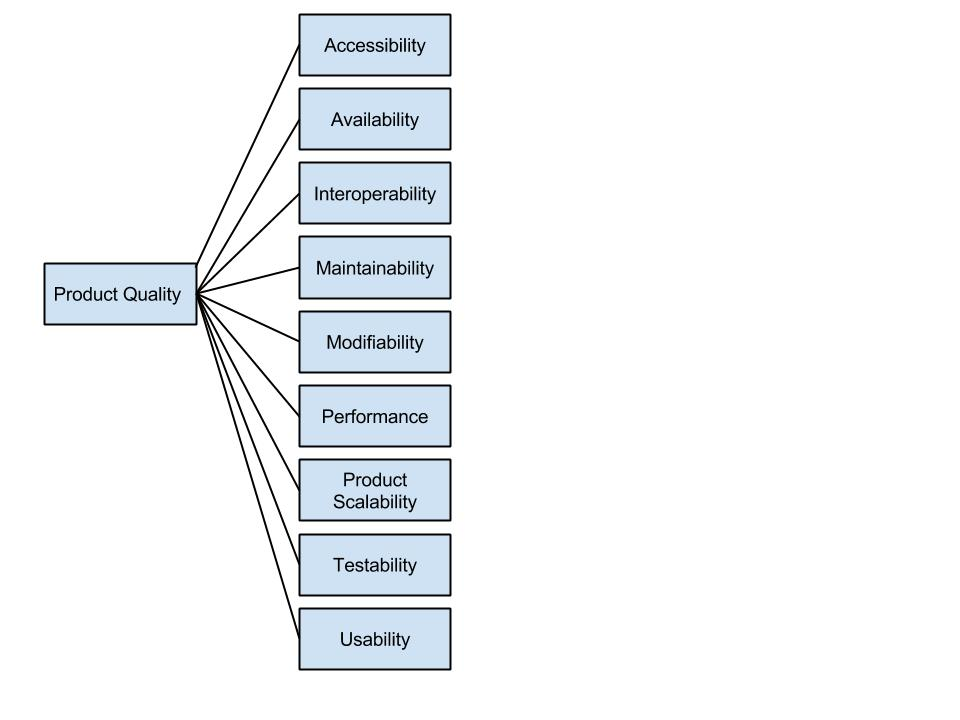
\includegraphics[scale=0.4]{images/qualityAttributes.jpg}
    \caption{Quality attributes.}
    \label{img:qualityAttributes}
    \end{center}
\end{figure}